%% =============================================================================
%% Projeto Base - Relatório de Estágio com abnTeX2
%% Customizado para a UNIJUÍ
%% Template desenvolvido e mantido por: Prof. Eldair F. Dornelles
%% A versão mais atualizada deste template pode ser obtida no GitHub:
%% https://github.com/dornelles/relatorio-de-estagio-template-latex
%% Qualquer sugestão de melhoria será bem vinda, 
%% Contato pelo e-mail: eldair.dornelles@unijui.edu.br
%% =============================================================================

\documentclass[
    12pt,               % tamanho da fonte
    oneside,            % para impressão frente e verso (use oneside para apenas frente)
    a4paper,            % tamanho do papel
    chapter=TITLE,      % títulos de capítulos em maiúsculas
    section=TITLE,      % títulos de seções em maiúsculas
    english,            % idioma adicional para hifenização
    brazil              % o último idioma é o principal do documento
]{abntex2}

% ==============================================================================
% PACOTES ESSENCIAIS
% ==============================================================================

% --- Codificação e fontes ---
\usepackage[T1]{fontenc}        % seleção de códigos de fonte
\usepackage[utf8]{inputenc}     % codificação do documento (conversão automática dos acentos)
% \usepackage{lmodern}          % comentado: a fonte agora está definida no arquivo unijui.sty

% --- Pacotes de citações ---
\usepackage[brazilian,hyperpageref]{backref}  % páginas com as citações na bibl
\usepackage[alf,bibjustif]{abntex2cite}        % citações padrão ABNT (bibjustif = referências justificadas)

% --- Pacotes matemáticos ---
\usepackage{amsmath}
\usepackage{amssymb}

% --- Pacotes gráficos ---
\usepackage{graphicx}           % inclusão de gráficos
% NOTA: NÃO usar \usepackage{float} com abnTeX2/memoir - conflita com \newfloat
\usepackage{subfig}             % subfiguras
\usepackage{pdfpages}           % inclusão de páginas PDF

% --- Pacotes de tabelas ---
\usepackage{booktabs}           % tabelas profissionais
\usepackage{multirow}           % células que ocupam várias linhas
\usepackage{longtable}          % tabelas longas (múltiplas páginas)
\usepackage{array}              % personalização de colunas

% --- Outros pacotes úteis ---
\usepackage{microtype}          % melhorias de justificação
\usepackage{indentfirst}        % indenta o primeiro parágrafo de cada seção
\usepackage{color}              % controle de cores
\usepackage{xcolor}             % cores avançadas
\usepackage{listings}           % listagens de código-fonte
\usepackage{enumitem}           % listas personalizadas
\usepackage{lipsum}             % geração de texto fictício (remover na versão final)
\usepackage{totcount}           % conta o total de floats (figuras, tabelas, etc.) no documento

% --- Customizações UNIJUÍ ---
\input{unijui.sty}

% ==============================================================================
% CONFIGURAÇÕES DO PACOTE BACKREF
% ==============================================================================
% Configurações do pacote backref
% Usado sem a opção hyperpageref de backref
\renewcommand{\backrefpagesname}{Citado na(s) página(s):~}
% Texto padrão antes do número das páginas
\renewcommand{\backref}{}
% Define os textos da citação
\renewcommand*{\backrefalt}[4]{
    \ifcase #1 %
        Nenhuma citação no texto.%
    \or
        Citado na página #2.%
    \else
        Citado #1 vezes nas páginas #2.%
    \fi}%

% ==============================================================================
% CONFIGURAÇÕES DE LISTAGENS DE CÓDIGO
% ==============================================================================
\lstset{
    basicstyle=\ttfamily\small,
    numbers=left,
    numberstyle=\tiny\color{gray},
    stepnumber=1,
    numbersep=8pt,
    backgroundcolor=\color{white},
    showspaces=false,
    showstringspaces=false,
    showtabs=false,
    frame=single,
    rulecolor=\color{black},
    tabsize=2,
    captionpos=b,
    breaklines=true,
    breakatwhitespace=false,
    keywordstyle=\color{blue}\bfseries,
    commentstyle=\color{green!60!black},
    stringstyle=\color{red},
    escapeinside={\%*}{*)},
    literate=
        {á}{{\'a}}1 {é}{{\'e}}1 {í}{{\'i}}1 {ó}{{\'o}}1 {ú}{{\'u}}1
        {Á}{{\'A}}1 {É}{{\'E}}1 {Í}{{\'I}}1 {Ó}{{\'O}}1 {Ú}{{\'U}}1
        {ã}{{\~a}}1 {õ}{{\~o}}1 {Ã}{{\~A}}1 {Õ}{{\~O}}1
        {ç}{{\c{c}}}1 {Ç}{{\c{C}}}1
        {ê}{{\^e}}1 {â}{{\^a}}1 {ô}{{\^o}}1
}

% ==============================================================================
% DADOS DO TRABALHO
% ==============================================================================

% --- Informações do documento (preencher conforme o trabalho) ---
\titulo{Automação da Geração de Propostas Comerciais em PDF com Django e \LaTeX}
\autor{Cristian dos Santos Siqueira}
\local{Santa Rosa/RS}
\data{2026}
\orientador{Prof. Manuel Osorio Binelo}
\instituicao{%
    Universidade Regional do Noroeste do\\[1mm]
    Estado do Rio Grande do Sul
}

% --- Informações específicas da UNIJUÍ (definidas no unijui.sty) ---
\campus{Santa Rosa}
\curso{Ciência da Computação}
\professordabanca{Prof(a). xxxx}
\datadabanca{XX}{XXX}{XXXX}

% --- Preâmbulo (texto da folha de rosto e aprovação) ---
% Não adicione ponto final do texto. Na folha de rosto o ponto irá aparecer automaticamente, 
% já na folha de aprovação ao invés de ponto irá aparecer uma vírgula, seguida do texto 
% "submetido à aprovação da banca examinadora composta pelos seguintes membros:"
\preambulo{Relatório de Estágio Supervisionado apresentado ao curso de Ciência da Computação da Universidade Regional do Noroeste do Estado do Rio Grande do Sul --- UNIJUÍ, como requisito parcial para a obtenção do grau de Bacharel em Ciência da Computação}

% --- Resumo e Abstract ---
\resumoemportugues{%
    Este relatório descreve as atividades desenvolvidas durante o estágio curricular obrigatório
    realizado na BIOTECNO Indústria e Comércio Ltda., empresa fabricante de equipamentos de
    refrigeração científica localizada em Santa Rosa, Rio Grande do Sul. O estágio foi realizado
    no contexto do sistema web interno da empresa, desenvolvido com o framework Django, que concentra
    os módulos de gestão comercial. O objetivo central do trabalho foi
    desenvolver um módulo de geração automatizada de propostas técnicas e comerciais em PDF,
    substituindo a abordagem anterior baseada na biblioteca PyLaTeX, que gerava documentos de forma
    estática e exigia intervenção direta no código-fonte a cada alteração de layout. A solução
    desenvolvida fundamenta-se em uma arquitetura orientada a layouts intercambiáveis: um novo modelo
    de dados, denominado \texttt{LayoutOrcamento}, foi projetado e implementado para permitir o
    cadastro e a ativação de templates de proposta diretamente pelo painel administrativo do Django,
    sem necessidade de alterações no código da aplicação. O template visual, elaborado por empresa de
    design contratada, foi codificado em LaTeX pelo estagiário e estruturado para ser processado pelo
    sistema de templates do Django, exigindo o tratamento adequado dos conflitos de sintaxe entre os
    dois sistemas. Na camada de lógica da aplicação, foram implementadas funções responsáveis pela
    resolução do diretório do layout ativo, pela montagem do contexto de dados, incluindo
    informações do cliente, itens do orçamento, descrições técnicas por conjunto de produto e
    condições comerciais e pela orquestração do pipeline de geração, que utiliza o compilador
    LuaLaTeX via \texttt{latexmk} para produzir o documento final. Ao término do período de estágio,
    o pipeline estava funcional em ambiente de desenvolvimento, com o template sendo renderizado e
    compilado corretamente, e a injeção das variáveis de contexto em fase de validação final antes
    da publicação em produção. O trabalho proporcionou a aplicação integrada de conhecimentos de
    Engenharia de Software, modelagem relacional, desenvolvimento web e composição tipográfica,
    consolidando competências técnicas e profissionais relevantes para a formação em Ciência da
    Computação.
}
% Instrução: Use letras minúsculas para as palavras-chave, separe-as com ponto e vírgula (;) e encerre a última com um ponto (.)
\palavraschaveemportugues{django; latex; geração de documentos; proposta comercial; engenharia de software; python.}


% ==============================================================================
% CONFIGURAÇÕES DE APARÊNCIA DO PDF FINAL
% ==============================================================================
\makeatletter
\hypersetup{
    pdftitle={\@title},
    pdfauthor={\@author},
    pdfsubject={\imprimirpreambulo},
    pdfcreator={LaTeX com abnTeX2},
    pdfkeywords={abnt}{latex}{abntex}{abntex2}{relatório de estágio},
    colorlinks=true,        % false: links em caixas; true: links coloridos
    linkcolor=black,        % cor dos links internos
    citecolor=black,        % cor dos links para bibliografias
    filecolor=black,        % cor dos links de arquivos
    urlcolor=black,         % cor dos links de URLs
    bookmarksdepth=4
}
\makeatother

% ==============================================================================
% ESPAÇAMENTOS ENTRE LINHAS E PARÁGRAFOS
% ==============================================================================
% O tamanho do parágrafo é dado por:
\setlength{\parindent}{1.3cm}
% Controle do espaçamento entre um parágrafo e outro:
\setlength{\parskip}{0.2cm}  % tente também \onelineskip

% ==============================================================================
% INÍCIO DO DOCUMENTO
% ==============================================================================
\begin{document}

% Seleciona o idioma do documento
\selectlanguage{brazil}

% Retira espaço extra obsoleto entre as frases
\frenchspacing

% --- Imprimir página de créditos e marca d'água ---
% \imprimirpaginadecreditos
% \imprimirmarcadagua

% ==========================================================================
% ELEMENTOS PRÉ-TEXTUAIS
% ==========================================================================
\pretextual

% --- Capa ---
\imprimircapa

% --- Folha de rosto ---
% (o * indica que haverá a ficha bibliográfica)
\imprimirfolhaderosto

% --- Ficha catalográfica (inserir PDF gerado pela biblioteca) ---
% \begin{fichacatalografica}
%     \includepdf{fig_ficha_catalografica.pdf}
% \end{fichacatalografica}

% --- Folha da banca ---
\imprimirfolhadabanca

% --- Agradecimentos ---
\begin{agradecimentos}
À \textbf{Lídia Linck} e ao \textbf{Nerci Linck}, pela oportunidade de realizar o estágio na
BIOTECNO Indústria e Comércio Ltda., pelo ambiente de trabalho que favorece o aprendizado e
pelo espaço dado para contribuir de forma técnica e significativa com os sistemas da
empresa.

Ao supervisor de estágio, \textbf{Gustavo Henrique Buuron}, pela orientação direta no
dia a dia do desenvolvimento, pela disponibilidade em discutir decisões técnicas e pela confiança
depositada ao longo de todo o período de estágio.

Ao professor orientador, \textbf{Prof. Manuel Osorio Binelo}, pelo acompanhamento acadêmico,
pelas contribuições à estruturação do trabalho e pelo suporte durante a elaboração deste relatório.

Ao \textbf{Prof. Eldair Fabricio Dornelles}, pelo desenvolvimento e disponibilização do template
\LaTeX{} utilizado neste relatório, publicado de forma aberta no GitHub e que foi fundamental
para a produção deste documento com qualidade tipográfica.
\end{agradecimentos}

% % --- Epígrafe ---
% \begin{epigrafe}
%     \vspace*{\fill}
%     \begin{flushright}
%         \textit{``A imaginação é mais importante que o conhecimento.''\\
%         (Albert Einstein)}
%     \end{flushright}
% \end{epigrafe}

% --- Resumo em português ---
\begin{resumo}
    \imprimirresumo
    \par
    \noindent \textbf{Palavras-chave}: \imprimirpalavraschave
\end{resumo}

% --- Lista de ilustrações (só aparece se houver figuras) ---
% Na primeira compilação os contadores podem ser 0; compile 2x para resultado correto.
\regtotcounter{figure}
\ifnum\totvalue{figure}>0
    \pdfbookmark[0]{\listfigurename}{lof}
    \listoffigures*
    \cleardoublepage
\fi

% --- Lista de quadros (só aparece se houver quadros) ---
\regtotcounter{quadro}
\ifnum\totvalue{quadro}>0
    \pdfbookmark[0]{\listofquadrosname}{loq}
    \listofquadros*
    \cleardoublepage
\fi

% --- Lista de tabelas (só aparece se houver tabelas) ---
\regtotcounter{table}
\ifnum\totvalue{table}>0
    \pdfbookmark[0]{\listtablename}{lot}
    \listoftables*
    \cleardoublepage
\fi

% --- Lista de abreviaturas e siglas ---
\begin{siglas}
    \item[ABNT]   Associação Brasileira de Normas Técnicas
    \item[ANVISA] Agência Nacional de Vigilância Sanitária
     \item[CNAE]   Classificação Nacional de Atividades Econômicas
    \item[CNPJ]   Cadastro Nacional da Pessoa Jurídica
    \item[FDA]    \textit{Food and Drug Administration}
    \item[HTTP]   \textit{Hypertext Transfer Protocol}
    \item[MVC]    \textit{Model-View-Controller}
    \item[MTV]    \textit{Model-Template-View}
    \item[ORM]    \textit{Object-Relational Mapper}
    \item[PDF]    \textit{Portable Document Format}
    \item[SQL]    \textit{Structured Query Language}
    \item[TCC]    Trabalho de Conclusão de Curso
    \item[UNIJUÍ] Universidade Regional do Noroeste do Estado do Rio Grande do Sul
\end{siglas}

% --- Lista de símbolos ---
%\begin{simbolos}
%    \item[$ \Gamma $] Letra grega Gama
%    \item[$ \Lambda $] Lambda
%\end{simbolos}

% --- Sumário ---
\pdfbookmark[0]{\contentsname}{toc}
\tableofcontents*
\cleardoublepage

% ==========================================================================
% ELEMENTOS TEXTUAIS
% ==========================================================================
\textual

% --- Inclusão dos capítulos ---
% ==============================================================================
% CAPÍTULO 1 - INTRODUÇÃO
% ==============================================================================

\chapter{Introdução}
\label{cap:introducao}

A transformação digital tem impactado de forma crescente os processos internos das empresas industriais,
tornando a automação de documentos e a integração entre sistemas operacionais cada vez mais estratégicas
para a competitividade. Nesse contexto, o desenvolvimento de software empresarial, em especial sistemas
de gestão customizados, emerge como uma disciplina central da Engenharia de Software, exigindo dos
profissionais habilidades que vão desde a modelagem de dados até a geração automatizada de documentos com
alto padrão visual.

A BIOTECNO Indústria e Comércio Ltda., empresa fabricante de equipamentos de refrigeração científica
localizada em Santa Rosa (RS), opera com um sistema web interno denominado Bioweb, desenvolvido em
Django. Dentro do módulo comercial do Bioweb, a geração de propostas técnicas e comerciais é uma das
atividades de maior impacto direto no relacionamento com clientes, pois o documento produzido representa
a empresa perante o mercado.

Até o início deste estágio, os orçamentos em PDF eram gerados por meio da biblioteca PyLaTeX, que
construía o documento de forma programática e estática, ou seja, qualquer alteração no layout da
proposta exigia modificação direta no código-fonte Python. Esse modelo limitava a capacidade de
atualização visual das propostas e criava dependência técnica para ajustes que, em essência, são decisões
de negócio e identidade visual. Paralelamente, a empresa contratou uma empresa de design para a criação
de um novo layout de proposta comercial, o qual precisava ser integrado ao sistema existente de forma
flexível e sustentável.

Este relatório descreve as atividades desenvolvidas ao longo do estágio curricular obrigatório realizado
na BIOTECNO, com foco na concepção e implementação de um sistema de geração automatizada de propostas
comerciais em PDF. O trabalho envolveu a codificação do template LaTeX a partir do layout entregue pela
empresa de design, a modelagem de um novo conjunto de entidades no banco de dados, e o desenvolvimento
da lógica de geração de documentos na camada de \textit{views} do Django com ênfase em uma arquitetura
que permita a troca de layouts diretamente pelo painel administrativo, sem necessidade de alterações no
código.

%-------------------------------------------------
% Justificativa
%-------------------------------------------------
\section{Justificativa}
\label{sec:justificativa}

A prática de estágio supervisionado constitui etapa fundamental na formação do profissional de Ciência da
Computação, pois permite a aplicação concreta dos conhecimentos construídos ao longo do curso em
problemas reais de complexidade e escala incompatíveis com o ambiente acadêmico isolado. A exposição a
decisões de arquitetura de software com impacto direto em processos de negócio desenvolve no estagiário
uma visão sistêmica que complementa a formação teórica.

Do ponto de vista acadêmico, o projeto demandou a aplicação integrada de conteúdos de Engenharia de
Software (modelagem de requisitos, padrões de projeto), Banco de Dados (modelagem relacional, migrações),
Desenvolvimento Web (arquitetura MVC/MTV, \textit{views} baseadas em função) e Sistemas de Composição
Tipográfica (\LaTeX{}), demonstrando a interdisciplinaridade inerente ao desenvolvimento de sistemas
reais. A necessidade de integrar dois sistemas com gramáticas conflitantes --- o motor de templates do
Django e a sintaxe do \LaTeX{} --- e de tomar decisões arquiteturais com impacto direto na
manutenibilidade do sistema são exemplos de desafios que a formação acadêmica prepara teoricamente,
mas que só se consolidam no contato com um ambiente produtivo real.

%-------------------------------------------------
% Objetivos
%-------------------------------------------------
\section{Objetivos}
\label{sec:objetivos}

\subsection{Objetivo Geral}
\label{subsec:objective-geral}

Desenvolver um módulo de geração automatizada de propostas técnicas e comerciais em PDF, integrado ao
sistema Django da BIOTECNO, com suporte a layouts intercambiáveis gerenciáveis pelo painel administrativo,
substituindo a abordagem estática anterior baseada na biblioteca PyLaTeX.

\subsection{Objetivos Específicos}
\label{subsec:objetivos-especificos}

\begin{alineas}
    \item Analisar o processo vigente de geração de orçamentos e levantar os requisitos funcionais e
    não funcionais do novo sistema;
    \item Traduzir o layout visual elaborado pela empresa de design para um template \LaTeX{} funcional,
    parametrizável via sistema de templates do Django;
    \item Modelar e implementar o modelo \texttt{LayoutOrcamento} no banco de dados, incluindo suporte
    ao upload de templates compactados e ao mecanismo de layout ativo único;
    \item Desenvolver as funções de resolução de diretório de layout, montagem de contexto e geração de
    PDF na camada de \textit{views} do Django, integrando o pipeline completo do banco de dados à
    entrega do documento ao navegador;
    \item Documentar o processo de desenvolvimento e os procedimentos necessários para manutenção
    futura da solução.
\end{alineas}

%-------------------------------------------------
% Estrutura do Trabalho
%-------------------------------------------------
\section{Estrutura do Trabalho}
\label{sec:estrutura}

Para melhor compreensão, este relatório está organizado em capítulos sequenciais. Além desta Introdução,
o \autoref{ch:apresentacao-empresa} apresenta o perfil da BIOTECNO Indústria e Comércio Ltda. e o
ambiente tecnológico em que o estágio foi realizado. O \autoref{cap:metodologia} descreve a sistemática
de trabalho adotada, as ferramentas utilizadas e a forma como as demandas foram gerenciadas ao longo do
período. O \autoref{ch:revisao-bibliografica} fundamenta tecnicamente o projeto, discutindo os principais
conceitos e tecnologias empregados. O \autoref{cap:desenvolvimento} detalha o processo completo de
análise, modelagem e implementação do sistema de geração de orçamentos. Por fim, o
\autoref{cap:consideracoes} apresenta as conclusões e perspectivas de trabalhos futuros.
% ==============================================================================
% CAPÍTULO 2 - APRESENTAÇÃO DA EMPRESA
% ==============================================================================

\chapter{Apresentação da Empresa}
\label{ch:apresentacao-empresa}

A BIOTECNO Indústria e Comércio Ltda. é uma empresa brasileira fabricante de refrigeradores e
freezers científicos, sediada em Santa Rosa, no noroeste do estado do Rio Grande do Sul. Com atuação
voltada ao mercado de saúde e pesquisa científica, a empresa desenvolve soluções para a conservação de
imunobiológicos, hemoderivados, medicamentos termolábeis e amostras laboratoriais, atendendo a um
público exigente quanto à precisão técnica e à conformidade regulatória. Este capítulo apresenta o
histórico da organização, seus pilares estratégicos e a estrutura tecnológica em que o estágio foi
realizado.

%-------------------------------------------------
\section{Histórico}
%-------------------------------------------------
\label{sec:historico}

A BIOTECNO foi fundada em 22 de maio de 2001, em Santa Rosa (RS), por um grupo de profissionais com
conhecimento técnico na área de refrigeração e uma visão clara das lacunas existentes no mercado
nacional de conservação de materiais biológicos. Desde os seus primeiros anos de operação, a empresa
orientou sua atuação ao desenvolvimento de câmaras científicas voltadas à cadeia de frio, segmento
que exige rigorosa estabilidade térmica e conformidade com normas sanitárias nacionais e internacionais.

Um dos marcos que consolidou a empresa no mercado nacional foi o desenvolvimento de uma linha de
câmaras para conservação de imunobiológicos, termolábeis e hemoderivados com capacidade de manter
operação durante períodos de ausência de energia elétrica, inovação inédita no país à época e que
atendeu a uma demanda crítica de postos de saúde, clínicas e hospitais localizados em regiões com
fornecimento elétrico instável. Essa inovação fez da BIOTECNO a marca de refrigeração científica
mais premiada do Brasil, com reconhecimento também em feiras e eventos internacionais do setor.

Com mais de duas décadas de trajetória, a empresa consolidou sua posição como referência nacional em
refrigeração médico-científica, com equipamentos registrados no Ministério da Saúde e certificados pela
\textit{U.S. Food and Drug Administration} (FDA), ampliando sua presença para o mercado
internacional. Atualmente, a BIOTECNO conta com mais de 20 anos de história desenvolvendo
soluções para a cadeia de frio, mantendo sua sede na Estrada Municipal João Hermes, 915,
bairro Glória, em Santa Rosa (RS), e uma filial ativa na mesma cidade.

%-------------------------------------------------
\section{Missão, Visão e Valores}
%-------------------------------------------------
\label{sec:missao-visao-valores}

Os pilares estratégicos da BIOTECNO refletem sua origem técnica e sua vocação para o mercado de saúde.
A missão da empresa é desenvolver e fabricar refrigeradores e freezers científicos de alta qualidade,
contribuindo para a conservação segura de materiais biológicos e para a proteção da saúde humana,
sintetizada em seu lema institucional \textit{Conserving Life}.

A visão é ser reconhecida como a principal referência brasileira em refrigeração científica, com
presença consolidada nos mercados nacional e internacional e portfólio alinhado às mais exigentes
normas regulatórias de saúde do mundo.

Os valores que orientam as práticas da organização incluem: inovação contínua, com investimento
permanente em pesquisa e desenvolvimento de produtos; qualidade técnica, expressa pela conformidade
com as normas da ANVISA e da FDA; proximidade com o cliente, com compromisso declarado de total
satisfação e disponibilização de diversos canais de atendimento; e responsabilidade com
a saúde pública, reconhecendo que os equipamentos fabricados integram diretamente a infraestrutura
de saúde de hospitais, farmácias, postos de vacinação e centros de pesquisa.

% ==============================================================================
% CAPÍTULO 3 - METODOLOGIA
% ==============================================================================

\chapter{Metodologia}
\label{cap:metodologia}

O estágio foi realizado de forma presencial nas dependências da BIOTECNO, com carga horária distribuída
ao longo da semana conforme acordo com o supervisor Gustavo Henrique Buuron. As demandas de
desenvolvimento foram conduzidas de maneira iterativa e incremental, próxima a uma abordagem ágil
informal: as tarefas eram discutidas com o supervisor, executadas em ciclos curtos e revisadas à medida
que os resultados parciais emergiam, permitindo ajustes contínuos de escopo e implementação.

A organização das atividades seguiu um fluxo composto pelas seguintes etapas: (1) compreensão do
problema ou requisito apresentado pelo supervisor; (2) análise do sistema existente, leitura de
\textit{models}, \textit{views} e templates já implementados, para entender o contexto de integração;
(3) implementação da solução, com testes manuais no ambiente de desenvolvimento; e (4) revisão conjunta
com o supervisor antes de integrar a funcionalidade à base de código principal.

As ferramentas e tecnologias centrais do projeto foram:

\begin{alineas}
    \item \textbf{Python} e \textbf{Django}: linguagem e framework base do sistema web da empresa,
    utilizados em todas as etapas de desenvolvimento \cite{django2024};
    \item \textbf{LaTeX} com compilador \textbf{LuaLaTeX} via \texttt{latexmk}: sistema de composição
    tipográfica utilizado para a geração dos documentos PDF \cite{latex2023};
    \item \textbf{PostgreSQL}: sistema gerenciador de banco de dados relacional utilizado pela aplicação;
    \item \textbf{Git}: controle de versão para rastreamento das alterações no código-fonte;
    \item \textbf{Django Admin}: interface administrativa nativa do Django, utilizada como ponto de
    gerenciamento dos layouts de orçamento.
\end{alineas}

A comunicação técnica com o supervisor ocorreu diariamente, permitindo que decisões de arquitetura 
como a escolha de resolver o layout ativo em tempo de geração em vez de vinculá-lo ao modelo
\texttt{Orcamento} fossem validadas antes de serem implementadas. Essa dinâmica reduziu retrabalho e
garantiu que a solução fosse coerente com as necessidades operacionais da empresa.
% ==============================================================================
% CAPÍTULO 4 - REVISÃO BIBLIOGRÁFICA
% ==============================================================================

\chapter{Revisão Bibliográfica}
\label{ch:revisao-bibliografica}

Este capítulo apresenta os fundamentos teóricos e tecnológicos que embasam o trabalho desenvolvido
durante o estágio. São abordados os principais conceitos relacionados ao desenvolvimento web com Django,
à geração de documentos com LaTeX e à modelagem de dados relacional, pilares sobre os quais a solução
de geração automatizada de propostas comerciais foi construída.

%-------------------------------------------------
\section{Django e o Padrão MTV}
%-------------------------------------------------
\label{sec:django}

Django é um \textit{framework} web de alto nível escrito em Python, projetado para facilitar o
desenvolvimento rápido de aplicações web seguras e de fácil manutenção \cite{django2024}. Sua arquitetura
segue o padrão MTV (\textit{Model-Template-View}), uma variação do amplamente conhecido MVC
(\textit{Model-View-Controller}), no qual o \textit{Model} define a estrutura dos dados e sua relação
com o banco de dados; o \textit{Template} é responsável pela apresentação, seja HTML, seja um documento
LaTeX, como utilizado neste projeto; e a \textit{View} concentra a lógica de negócio, recebendo
requisições HTTP, consultando os modelos e retornando uma resposta ao cliente \cite{holovaty2009}.

Um dos componentes centrais do Django utilizado neste projeto é o ORM (\textit{Object-Relational
Mapper}), que permite interagir com o banco de dados por meio de classes Python, abstraindo a escrita
de SQL. Cada modelo Django é uma subclasse de \texttt{django.db.models.Model}, e seus atributos
correspondem às colunas de uma tabela relacional. As migrações, geradas automaticamente pelo comando
\texttt{makemigrations}, traduzem alterações nos modelos em operações de banco de dados reproduzíveis e
controladas por versão \cite{django2024}.

O sistema de \textit{templates} do Django suporta uma linguagem própria de marcação que permite
interpolação de variáveis, estruturas de controle (\textit{if}, \textit{for}) e herança de templates.
Por padrão, os delimitadores dessa linguagem são chaves duplas para variáveis e blocos
percentual-chave para \textit{tags}, o que pode gerar conflitos com a sintaxe do LaTeX, cujo
caractere de percentual tem função de comentário e cujas chaves são usadas extensivamente como
delimitadores de comandos. Esse conflito demanda atenção durante o desenvolvimento de templates LaTeX
processados pelo Django.

%-------------------------------------------------
\section{LaTeX e Geração de Documentos}
%-------------------------------------------------
\label{sec:latex}

LaTeX é um sistema de preparação de documentos baseado no programa de composição tipográfica TeX,
desenvolvido por Donald Knuth \cite{knuth1984}. Diferentemente de editores \textit{WYSIWYG}
(\textit{What You See Is What You Get}), no LaTeX o autor descreve a estrutura e o conteúdo do documento
por meio de comandos textuais, e o sistema se encarrega da diagramação final, resultando em documentos
com qualidade tipográfica superior \cite{lamport1994}.

Para a compilação de documentos LaTeX em arquivos PDF, este projeto utiliza o compilador
\textbf{LuaLaTeX}, variante moderna do LaTeX com suporte nativo a Unicode e a fontes OpenType, em
conjunto com o utilitário \texttt{latexmk}, que automatiza o processo de compilação, executando o
compilador quantas vezes forem necessárias para resolver referências cruzadas, sumários e outros
elementos que dependem de múltiplas passagens \cite{latex2023}.

A abordagem adotada neste projeto, renderizar um template \texttt{.tex} com o sistema de templates do
Django e, em seguida, compilá-lo com \texttt{latexmk}, é uma estratégia consolidada para geração de
PDFs com alto controle tipográfico em aplicações web, especialmente quando o documento exige layout
complexo, como tabelas posicionadas com precisão, imagens integradas e fontes customizadas.

%-------------------------------------------------
\section{Modelagem Relacional e Django ORM}
%-------------------------------------------------
\label{sec:modelagem-relacional}

A modelagem relacional é a base sobre a qual os sistemas de informação organizam e persistem seus dados.
No contexto do Django, a definição dos modelos determina diretamente a estrutura do banco de dados e,
consequentemente, as possibilidades de consulta e relacionamento entre entidades \cite{elmasri2011}.

Neste projeto, um aspecto relevante da modelagem é a decisão de \textbf{não} vincular o layout de
orçamento diretamente ao modelo \texttt{Orcamento} por meio de uma chave estrangeira. Em vez disso, o
sistema resolve o layout ativo em tempo de geração, consultando o modelo \texttt{LayoutOrcamento} pelo
campo \texttt{is\_active}. Essa decisão arquitetural segue o princípio de baixo acoplamento
(\textit{loose coupling}): o modelo de negócio central (\texttt{Orcamento}) permanece desacoplado das
decisões de apresentação (layout), facilitando a evolução independente de ambos \cite{martin2002}.

O campo \texttt{AutoSlugField}, fornecido pela biblioteca \texttt{django-autoslug}, gera
automaticamente um identificador textual único a partir de outro campo do modelo — neste caso, a
descrição do layout — sem requerer intervenção manual, o que simplifica a identificação de registros em
rotas e na interface administrativa.

%-------------------------------------------------
\section{Arquitetura de Software e Boas Práticas}
%-------------------------------------------------
\label{sec:arquitetura}

O princípio da separação de responsabilidades (\textit{Separation of Concerns}) orienta a organização do
código em camadas com papéis bem definidos \cite{dijkstra1982}. No contexto deste projeto, ele se
manifesta na divisão entre: (a) a camada de modelos, responsável pela persistência e pela lógica de
dados; (b) a camada de \textit{views}, responsável pela orquestração, ou seja, a resolução do layout ativo, montagem
do contexto e acionamento do compilador; e (c) a camada de templates, responsável exclusivamente pela
estrutura visual do documento LaTeX.

Essa separação garante que alterações no layout não exijam modificações na lógica da \textit{view}, e
que mudanças nas regras de negócio não impactem a estrutura do template, reduzindo o custo de
manutenção e aumentando a testabilidade do sistema \cite{martin2002}.
% ==============================================================================
% CAPÍTULO 5 - DESENVOLVIMENTO
% ==============================================================================

\chapter{Desenvolvimento}
\label{cap:desenvolvimento}

Este capítulo descreve o processo de análise, modelagem e implementação do módulo de geração
automatizada de propostas técnicas e comerciais (orçamentos) em PDF. O trabalho partiu do diagnóstico
do sistema legado, passou pela concepção de uma nova arquitetura orientada a layouts intercambiáveis e
chegou à implementação de um pipeline completo, do banco de dados à entrega do arquivo PDF ao
navegador.

%-------------------------------------------------
\section{Análise e Levantamento de Requisitos}
%-------------------------------------------------
\label{sec:requisitos}

O processo de levantamento de requisitos foi conduzido por meio de reuniões com o supervisor de estágio
e da análise direta do sistema existente. A inspeção do código legado revelou que a geração de
orçamentos era realizada pela função \texttt{generate\_orcamento}, localizada no módulo
\texttt{comercial/latex.py}, que utilizava a biblioteca PyLaTeX para construir o documento PDF
programaticamente, adicionando tabelas, seções e formatações por meio de chamadas de função Python.
Embora funcional, essa abordagem apresentava limitações estruturais relevantes:

\begin{alineas}
    \item O layout do documento estava \textbf{codificado diretamente no código Python}, impossibilitando
    alterações visuais sem intervenção de desenvolvedor;
    \item Não havia suporte a \textbf{múltiplos layouts}, qualquer nova identidade visual exigia a
    reescrita da função de geração;
    \item A inclusão de \textbf{descrições técnicas dos equipamentos} por conjunto (componente de
    produto) não era contemplada de forma sistemática, prejudicando a completude da proposta.
\end{alineas}

Simultaneamente, a empresa contratou uma empresa de design para elaborar um novo modelo visual de
proposta comercial. Esse layout foi entregue como referência visual (não como arquivo LaTeX), cabendo ao
estagiário a sua codificação no formato \texttt{.tex}.

A partir dessa análise, foram definidos os seguintes requisitos:

\textbf{Requisitos Funcionais:}
\begin{alineas}
    \item O sistema deve permitir o cadastro de layouts de orçamento via painel administrativo do Django,
    com upload do template compactado em formato \texttt{.zip};
    \item Apenas um layout pode estar ativo por vez; a ativação de um novo layout deve desativar
    automaticamente o anterior;
    \item A geração do PDF deve utilizar o layout ativo no momento da requisição, sem necessidade de
    configuração manual;
    \item O documento gerado deve incluir: informações cadastrais do cliente, tabela de equipamentos com
    valores, descrições técnicas por conjunto de produto, imagens dos equipamentos e condições comerciais;
    \item O sistema deve ser compatível com orçamentos contendo múltiplos equipamentos, cada um com sua
    própria composição de conjuntos e opcionais.
\end{alineas}

\textbf{Requisitos Não Funcionais:}
\begin{alineas}
    \item A solução deve ser implementada dentro do \textit{framework} Django, seguindo os padrões já
    estabelecidos no sistema da empresa;
    \item O template LaTeX deve ser processado pelo sistema de templates do Django, exigindo tratamento
    adequado dos conflitos de sintaxe entre os dois sistemas;
    \item O compilador utilizado deve ser o LuaLaTeX via \texttt{latexmk}, padrão já adotado em outros
    módulos do sistema;
    \item A troca de layout não deve exigir alterações no código-fonte da aplicação.
\end{alineas}

%-------------------------------------------------
\section{Modelagem}
%-------------------------------------------------
\label{sec:modelagem}

\subsection{Contexto dos Modelos Existentes}

O sistema comercial já possuía os seguintes modelos centrais para o processo de orçamento:

\begin{alineas}
    \item \texttt{Orcamento}: representa a proposta comercial, com número de série, cliente, vendedor,
    versão e status;
    \item \texttt{OrcamentoEquipamento}: representa cada item do orçamento, armazenando o campo
    \texttt{equipamentodetail} --- uma cadeia de códigos de conjuntos de produto separados por ponto, que
    define a composição técnica do equipamento;
    \item \texttt{OrcamentoCondicoes}: armazena as condições comerciais da proposta (prazo, frete,
    garantia, pagamento);
    \item \texttt{DescricaoOrcamento\_Conjunto}: associa conjuntos de produto a textos descritivos
    utilizados nas propostas, com suporte a prioridade e configuração de chave;
    \item \texttt{RegraImagem\_Conjunto}: associa conjuntos de produto a imagens representativas,
    utilizadas no documento.
\end{alineas}

Os dois últimos modelos são detalhados nas subseções a seguir, pois receberam extensões diretas
durante o desenvolvimento.

\subsubsection{Modelo DescricaoOrcamento\_Conjunto}

O modelo \texttt{DescricaoOrcamento\_Conjunto} já existia no sistema e é responsável por vincular
textos descritivos a conjuntos de produto. Cada registro associa um ou mais conjuntos (relação
muitos-para-muitos) a um identificador curto (\texttt{orcamento\_desc}), um texto longo opcional
(\texttt{description}), uma configuração de chave (\texttt{config\_chave}) e um campo de
prioridade para ordenação.

No contexto deste projeto, duas contribuições foram realizadas sobre esse modelo: a adição de
uma chave estrangeira opcional para \texttt{LayoutOrcamento}, permitindo vincular descrições a
um layout específico; e a implementação do método \texttt{atende\_conjuntos(codes\_item)}, que
verifica se o registro é aplicável a um dado equipamento, agrupa os conjuntos vinculados por
configuração e retorna verdadeiro somente se \texttt{codes\_item} possui interseção com todos os
grupos, garantindo que apenas descrições pertinentes ao equipamento sejam incluídas na proposta.
A \autoref{fig:modelo-descricao} ilustra a estrutura e a lógica do modelo.

\begin{figure}[htb]
    \caption{\label{fig:modelo-descricao}Estrutura e lógica do modelo \texttt{DescricaoOrcamento\_Conjunto}}
    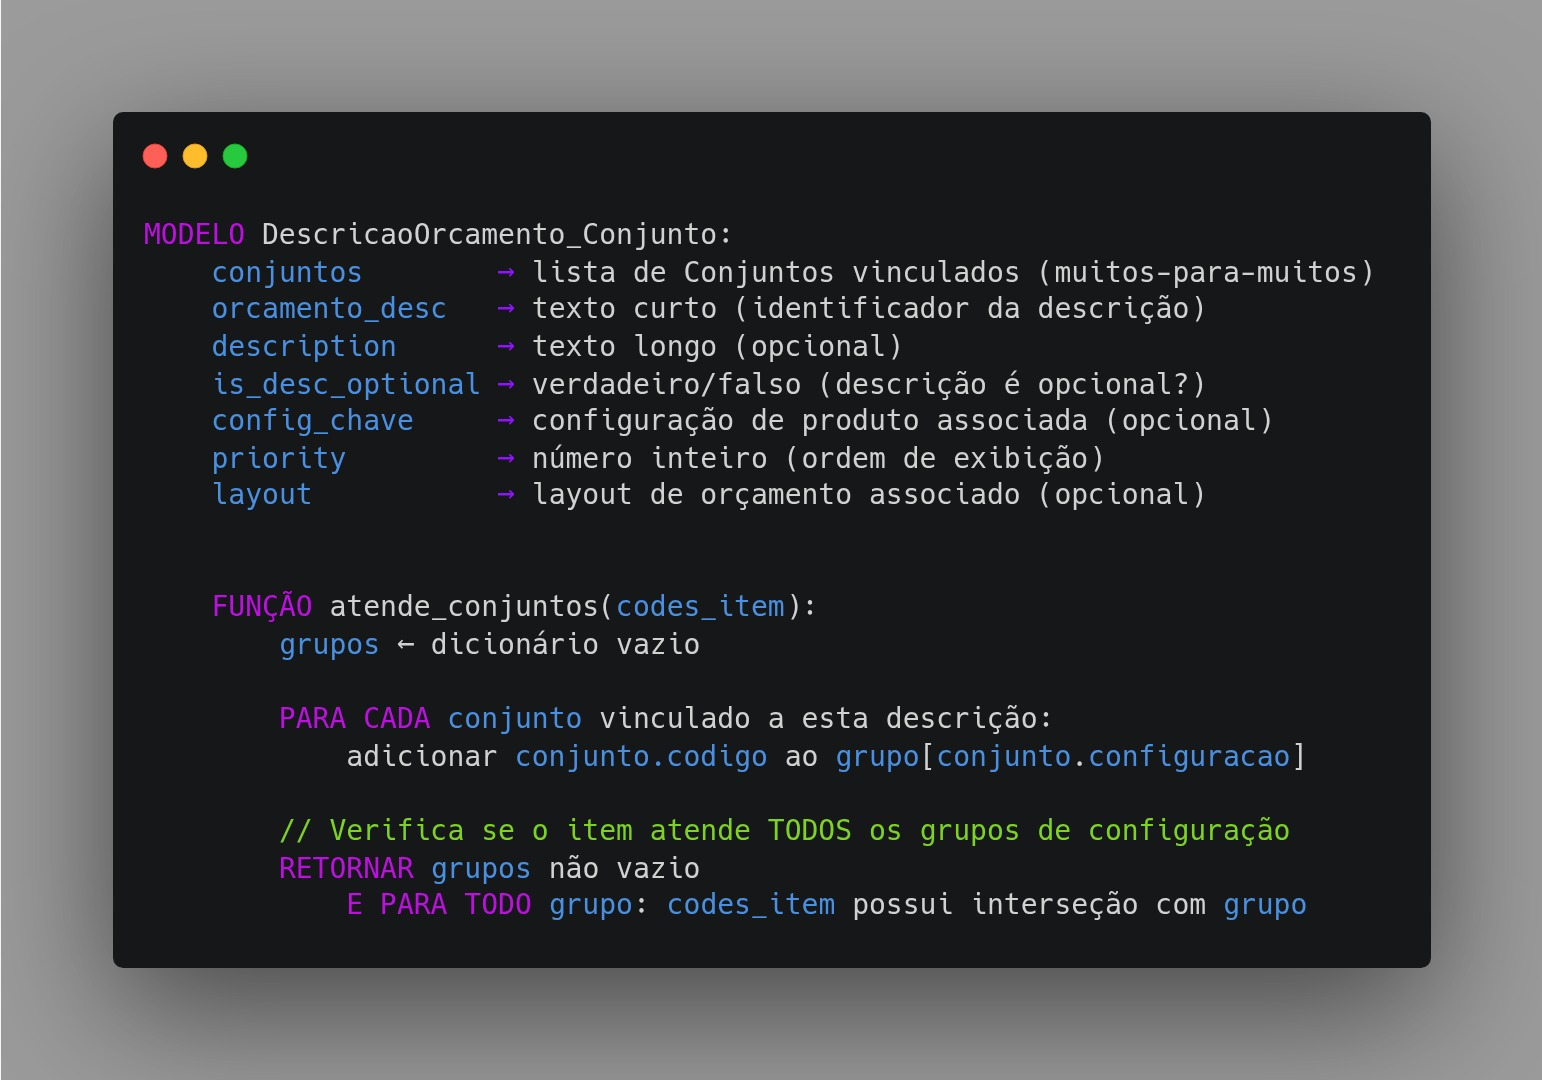
\includegraphics[width=0.85\textwidth]{figuras/05-desenvolvimento/Pseudo Código/Modelo descriçãoOrcamento_Conjunto.jpeg}
    \legend{Fonte: Própria do autor (2026), elaborado com Carbon (carbon.now.sh).}
\end{figure}

\subsubsection{Modelo RegraImagem\_Conjunto}

O modelo \texttt{RegraImagem\_Conjunto} segue estrutura análoga ao anterior, já existindo anteriormente, porém voltado
a imagens representativas dos equipamentos. Cada registro vincula um ou mais conjuntos ao
arquivo de imagem (\texttt{image}), a um identificador (\texttt{orcamento\_desc}) e a uma URL
opcional (\texttt{link}). O método \texttt{atende\_imagem(codes\_item)} aplica a mesma lógica
de interseção por grupos de configuração para determinar se a imagem é pertinente ao equipamento
em questão. A \autoref{fig:modelo-regraImagem} apresenta a estrutura do modelo.

\begin{figure}[htb]
    \caption{\label{fig:modelo-regraImagem}Estrutura e lógica do modelo \texttt{RegraImagem\_Conjunto}}
    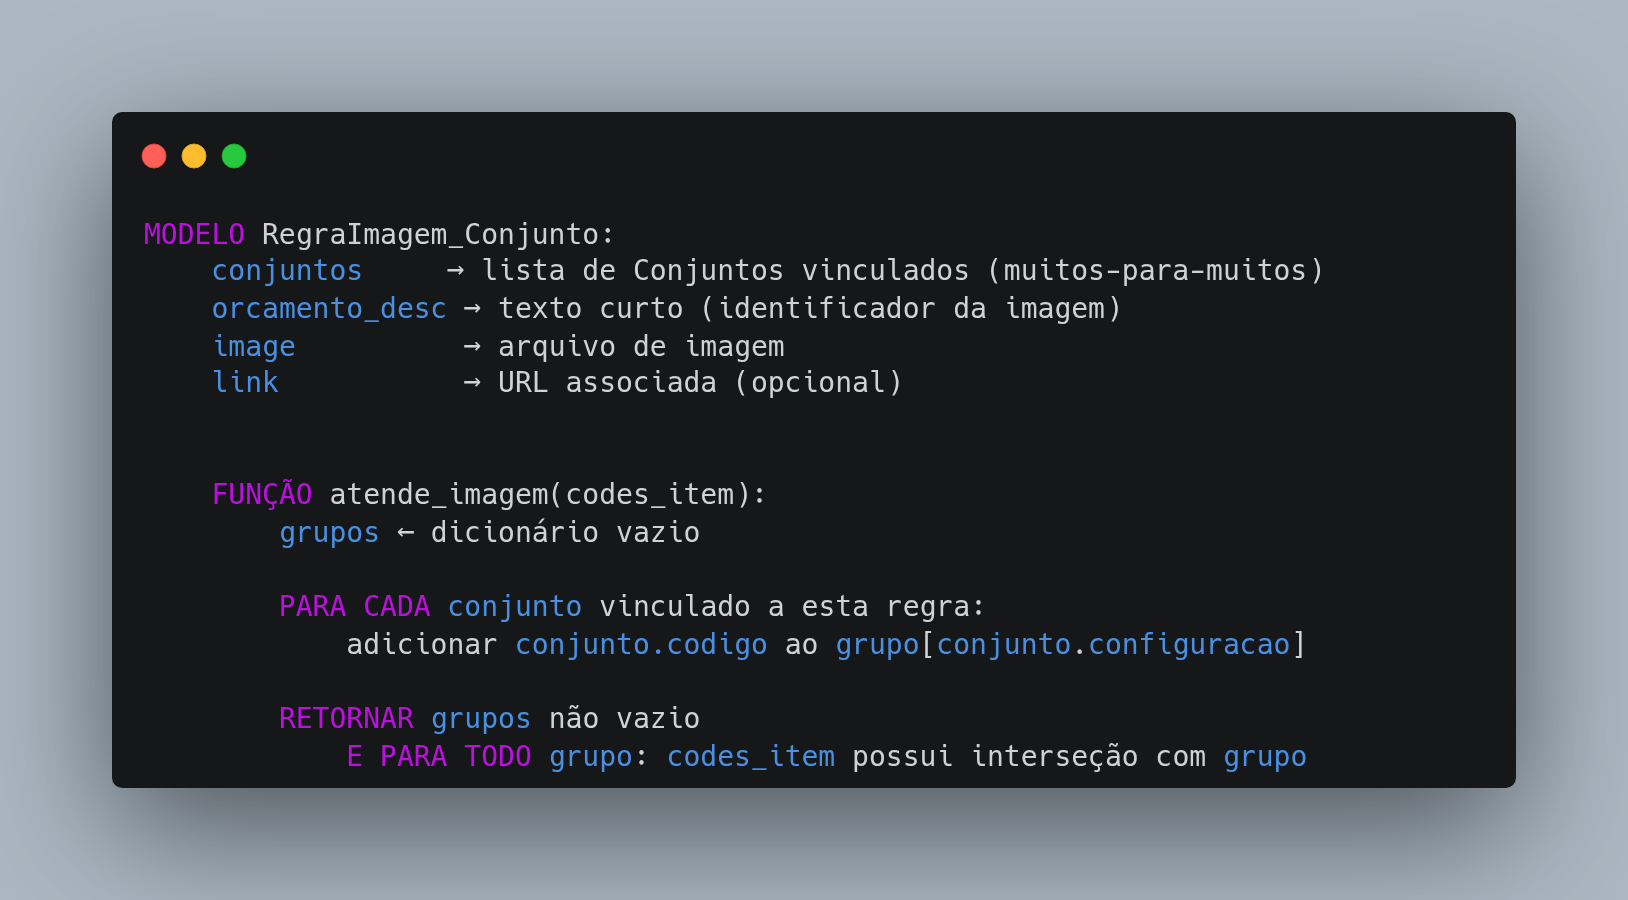
\includegraphics[width=0.85\textwidth]{figuras/05-desenvolvimento/Pseudo Código/ModeloRegraImagem.png}
    \legend{Fonte: Própria do autor (2026), elaborado com Carbon (carbon.now.sh).}
\end{figure}

\subsection{Novo Modelo: LayoutOrcamento}

Para suportar layouts intercambiáveis, foi projetado e implementado o modelo \texttt{LayoutOrcamento},
cuja estrutura é apresentada na \autoref{fig:modelo-layout} e detalhada no
Quadro~\ref{qdr:layout-orcamento}.

\begin{figure}[htb]
    \caption{\label{fig:modelo-layout}Estrutura e comportamento do modelo \texttt{LayoutOrcamento}}
    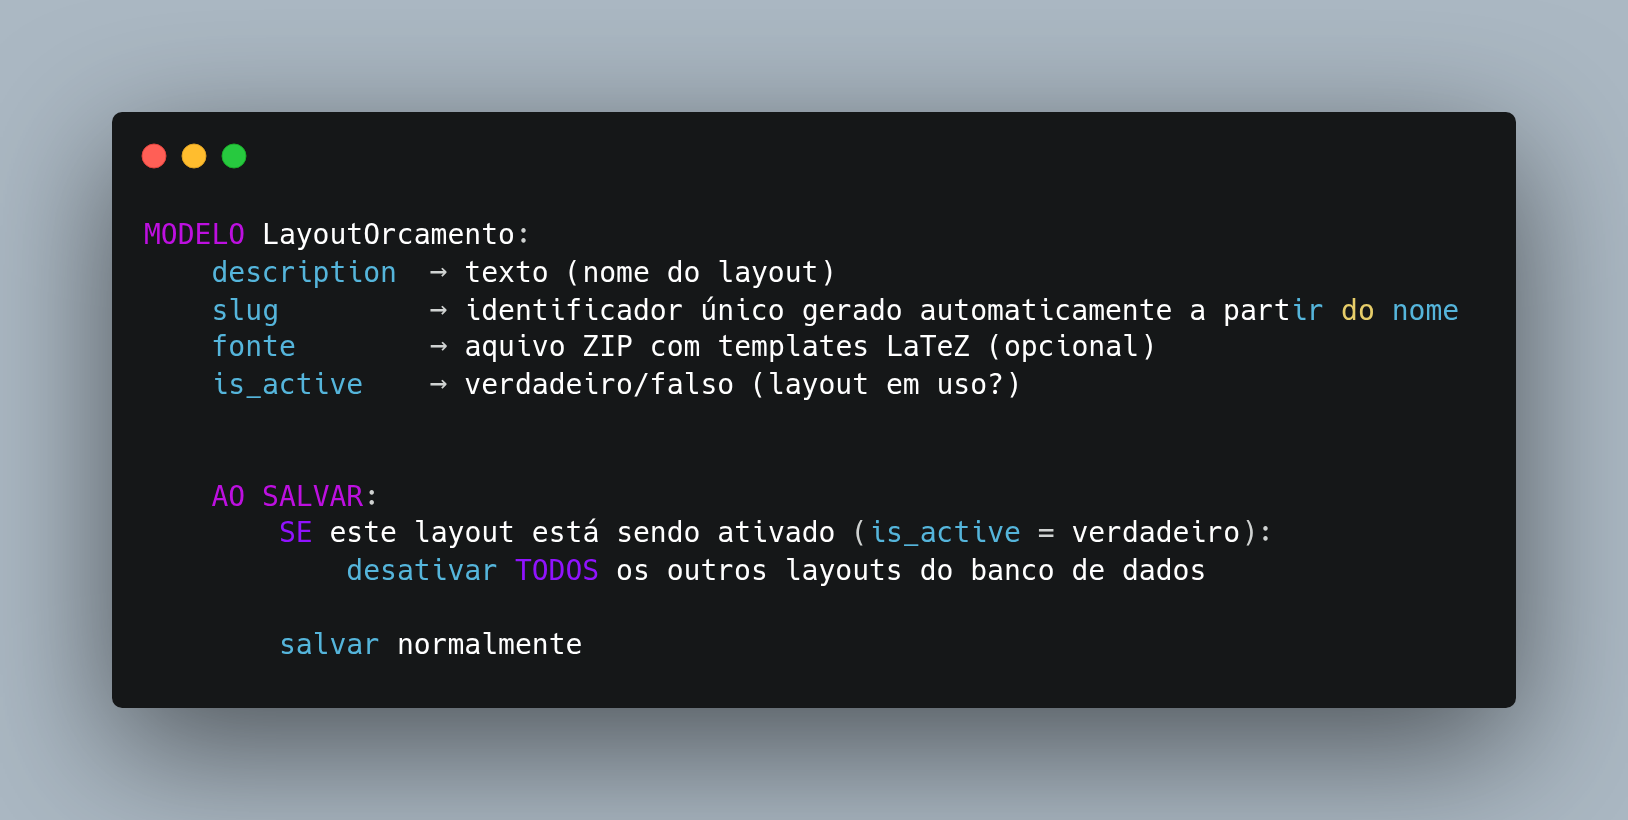
\includegraphics[width=0.75\textwidth]{figuras/05-desenvolvimento/Pseudo Código/ModeloLayoutOrcamento.png}
    \legend{Fonte: Própria do autor (2026), elaborado com Carbon (carbon.now.sh).}
\end{figure}

\begin{quadro}[htb]
    \caption{\label{qdr:layout-orcamento}Campos do modelo \texttt{LayoutOrcamento}}
    \begin{tabular}{|l|l|p{7cm}|}
        \hline
        \textbf{Campo} & \textbf{Tipo} & \textbf{Descrição} \\
        \hline
        \texttt{description} & \texttt{CharField} & Nome descritivo do layout \\
        \hline
        \texttt{slug} & \texttt{AutoSlugField} & Identificador único gerado a partir de \texttt{description} \\
        \hline
        \texttt{fonte} & \texttt{FileField} & Arquivo \texttt{.zip} contendo o template LaTeX e seus assets \\
        \hline
        \texttt{is\_active} & \texttt{BooleanField} & Indica se este é o layout em uso \\
        \hline
    \end{tabular}
    \legend{Fonte: Própria do autor (2026), elaborado com Carbon (carbon.now.sh).}
\end{quadro}

Uma decisão central de modelagem foi \textbf{não incluir} uma chave estrangeira de
\texttt{LayoutOrcamento} no modelo \texttt{Orcamento}. Essa escolha mantém o modelo de negócio
desacoplado das decisões de apresentação: o layout ativo é resolvido em tempo de geração,
por meio de uma consulta direta ao registro marcado como ativo, e não é persistido no orçamento.
Isso significa que diferentes gerações do mesmo orçamento podem utilizar layouts distintos,
conforme o layout ativo no momento --- comportamento adequado à realidade operacional da empresa,
onde a troca de layout é uma decisão de identidade visual global, não individual por proposta.

Os modelos \texttt{DescricaoOrcamento\_Conjunto} e \texttt{RegraImagem\_Conjunto} receberam
chaves estrangeiras opcionais para \texttt{LayoutOrcamento}, permitindo que descrições e imagens
sejam vinculadas a um layout específico. O sistema aplica um filtro com fallback: retorna registros
do layout ativo ou, na ausência, registros sem layout definido --- garantindo compatibilidade com
dados cadastrados antes da implementação do novo sistema.

O mecanismo de layout único ativo é garantido pelo método \texttt{save()} sobrescrito no modelo:
ao ativar um layout, todos os demais são automaticamente desativados antes da persistência do
registro, conforme ilustrado na \autoref{fig:modelo-layout}.

%-------------------------------------------------
\section{Implementação}
%-------------------------------------------------
\label{sec:implementacao}

A implementação foi dividida em três frentes interdependentes: (a) a codificação do template LaTeX;
(b) o desenvolvimento das funções de suporte na \textit{view}; e (c) a integração do pipeline completo
de geração de PDF.

\subsection{Codificação do Template LaTeX}

O layout visual elaborado pela empresa de design foi traduzido para um arquivo \texttt{main.tex}
estruturado para ser processado pelo sistema de templates do Django. Esse processo exigiu atenção
especial ao \textbf{conflito de delimitadores} entre os dois sistemas: o LaTeX utiliza extensivamente
o caractere de percentual como início de comentário e chaves como delimitadores de argumentos de
comandos, enquanto o Django utiliza chaves duplas para variáveis e blocos percentual-chave para
\textit{tags} de controle.

A solução adotada, já consolidada em outros módulos do sistema, como \texttt{viewsinspecao.py},
consiste em configurar o motor de templates com delimitadores customizados, substituindo a sintaxe
padrão do Django por sequências que não colidem com a gramática do LaTeX. Essa abordagem permite que
o arquivo \texttt{.tex} seja ao mesmo tempo um template Django válido e um documento LaTeX
sintaticamente correto.

O template é organizado em seções que correspondem às partes visuais do documento:

\begin{alineas}
    \item \textbf{Cabeçalho}: logotipo da empresa e identificação da proposta;
    \item \textbf{Informações cadastrais}: dados do cliente (razão social, CNPJ, município, contato);
    \item \textbf{Tabela de equipamentos}: itens do orçamento com quantidade, valor unitário e
    valor total;
    \item \textbf{Descrições técnicas}: para cada equipamento, as descrições dos conjuntos que o
    compõem são listadas em formato de tabela com identificadores de atributo e valores;
    \item \textbf{Imagens dos equipamentos}: imagens associadas aos conjuntos via
    \texttt{RegraImagem\_Conjunto};
    \item \textbf{Condições de fornecimento}: pagamento, frete, garantia, prazo e serviços inclusos;
    \item \textbf{Rodapé}: dados de contato e assinatura do consultor.
\end{alineas}

\begin{figure}[htb]
    \caption{\label{fig:modelo-regraImagem}Estrutura e lógica do template \texttt{main.tex}}
    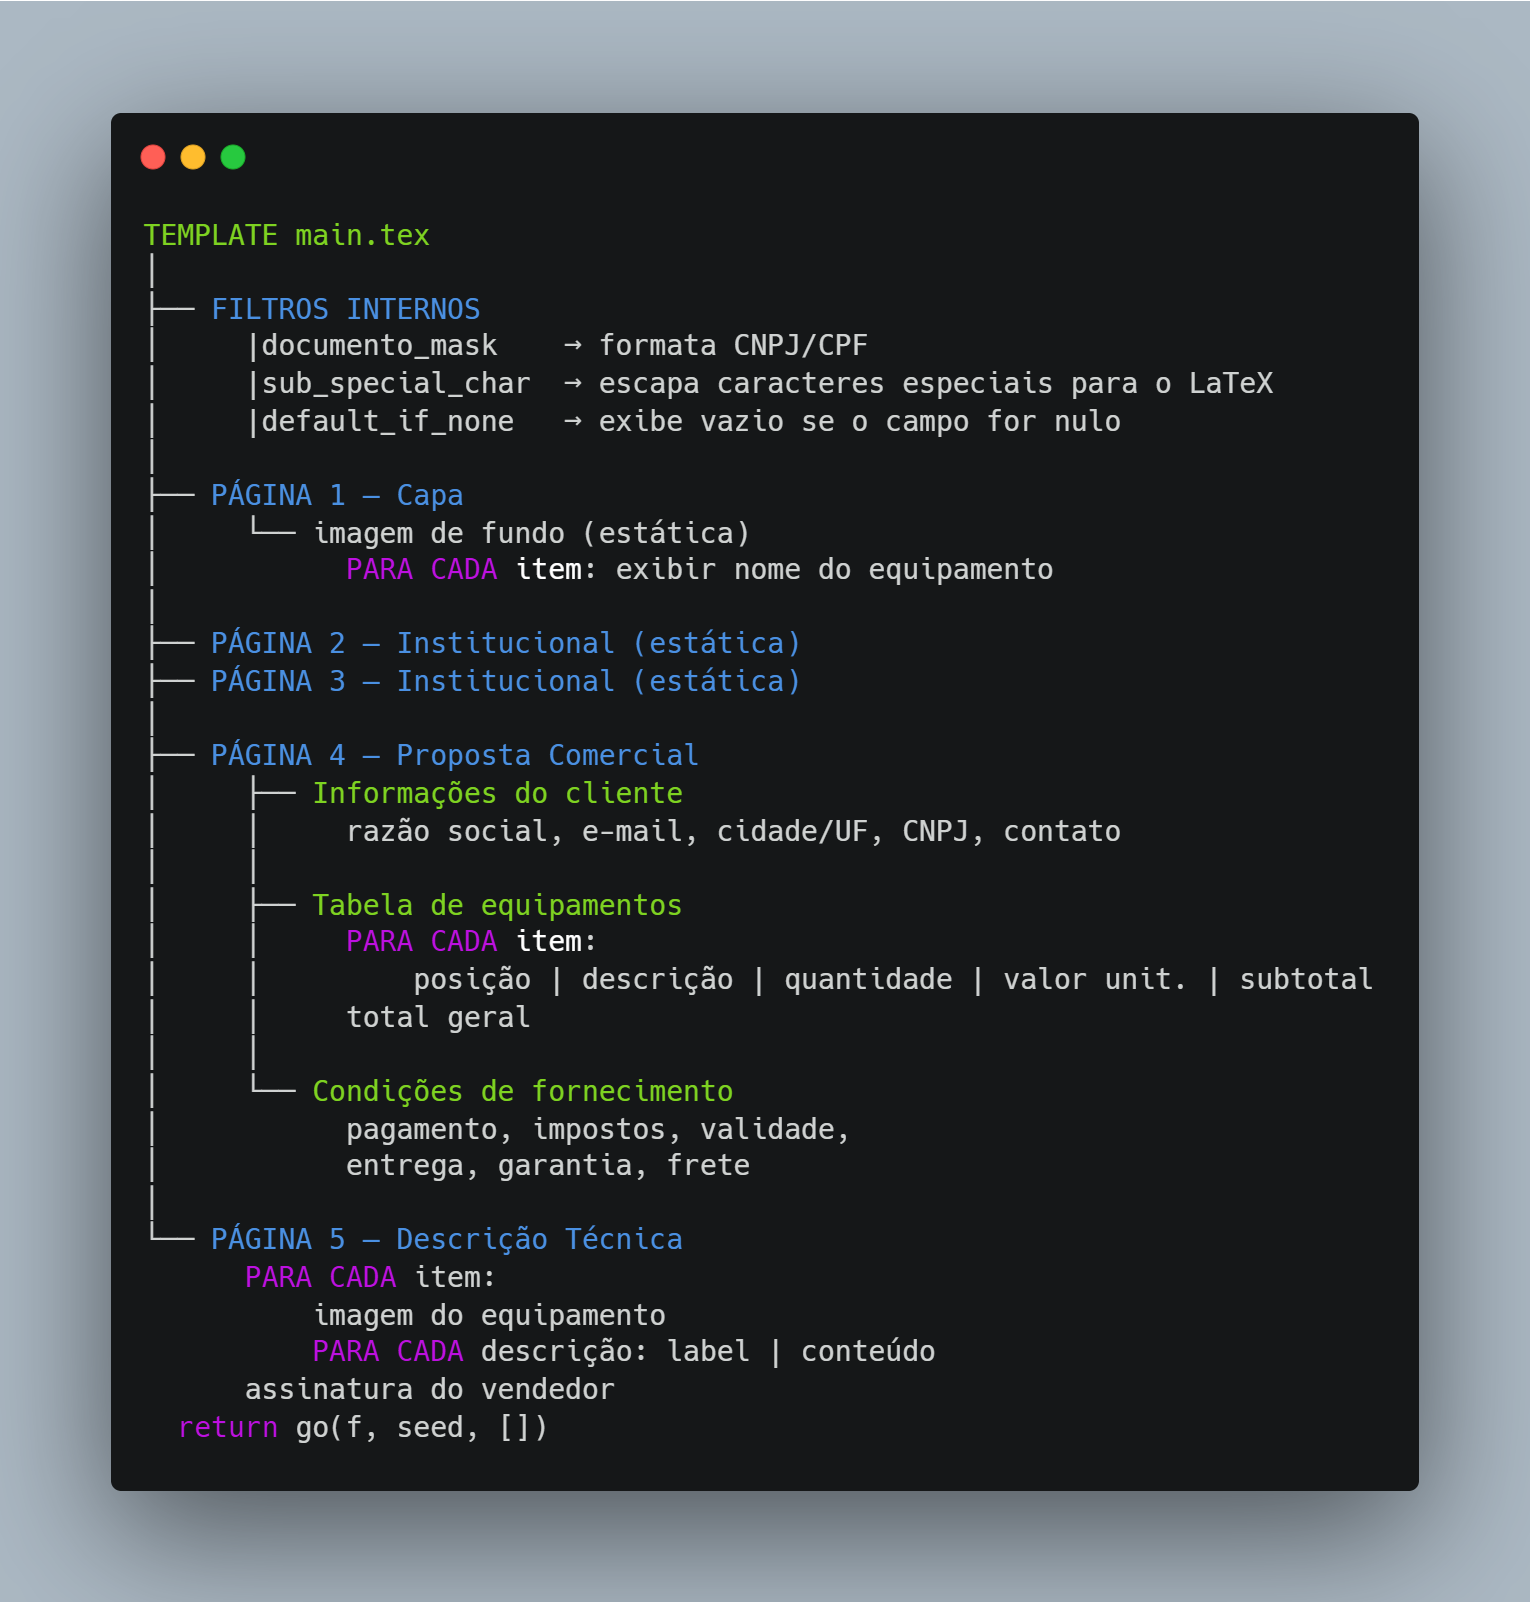
\includegraphics[width=0.85\textwidth]{figuras/05-desenvolvimento/Pseudo Código/TEX.png}
    \legend{Fonte: Própria do autor (2026), elaborado com Carbon (carbon.now.sh).}
\end{figure}

\subsection{Funções da \textit{View}}

Na camada de \textit{views}, foram implementadas três funções principais que compõem o pipeline de
geração, descritas a seguir.

\subsubsection{Função montar\_contexto\_orcamento\_layout}

A função \texttt{montar\_contexto\_orcamento\_layout} é responsável por construir o dicionário de
dados que será injetado no template LaTeX. Recebe o orçamento e a versão como parâmetros e,
internamente, resolve o layout ativo, as condições comerciais e os equipamentos vinculados ao
orçamento. Para cada equipamento, os códigos de conjuntos são extraídos do campo
\texttt{equipamentodetail} e utilizados para filtrar as descrições e imagens aplicáveis, por meio
dos métodos \texttt{atende\_conjuntos} e \texttt{atende\_imagem} descritos anteriormente.
As descrições são pré-carregadas com filtro de fallback --- layout ativo ou sem layout definido ---
e ordenadas por prioridade. O contexto retornado contém todos os dados necessários para a
renderização completa do documento, sem lógica de apresentação embutida.
A \autoref{fig:funcao-contexto} apresenta o pseudocódigo da função.

\begin{figure}[htb]
    \caption{\label{fig:funcao-contexto}Estrutura e lógica da função \texttt{montar\_contexto\_orcamento\_layout}}
    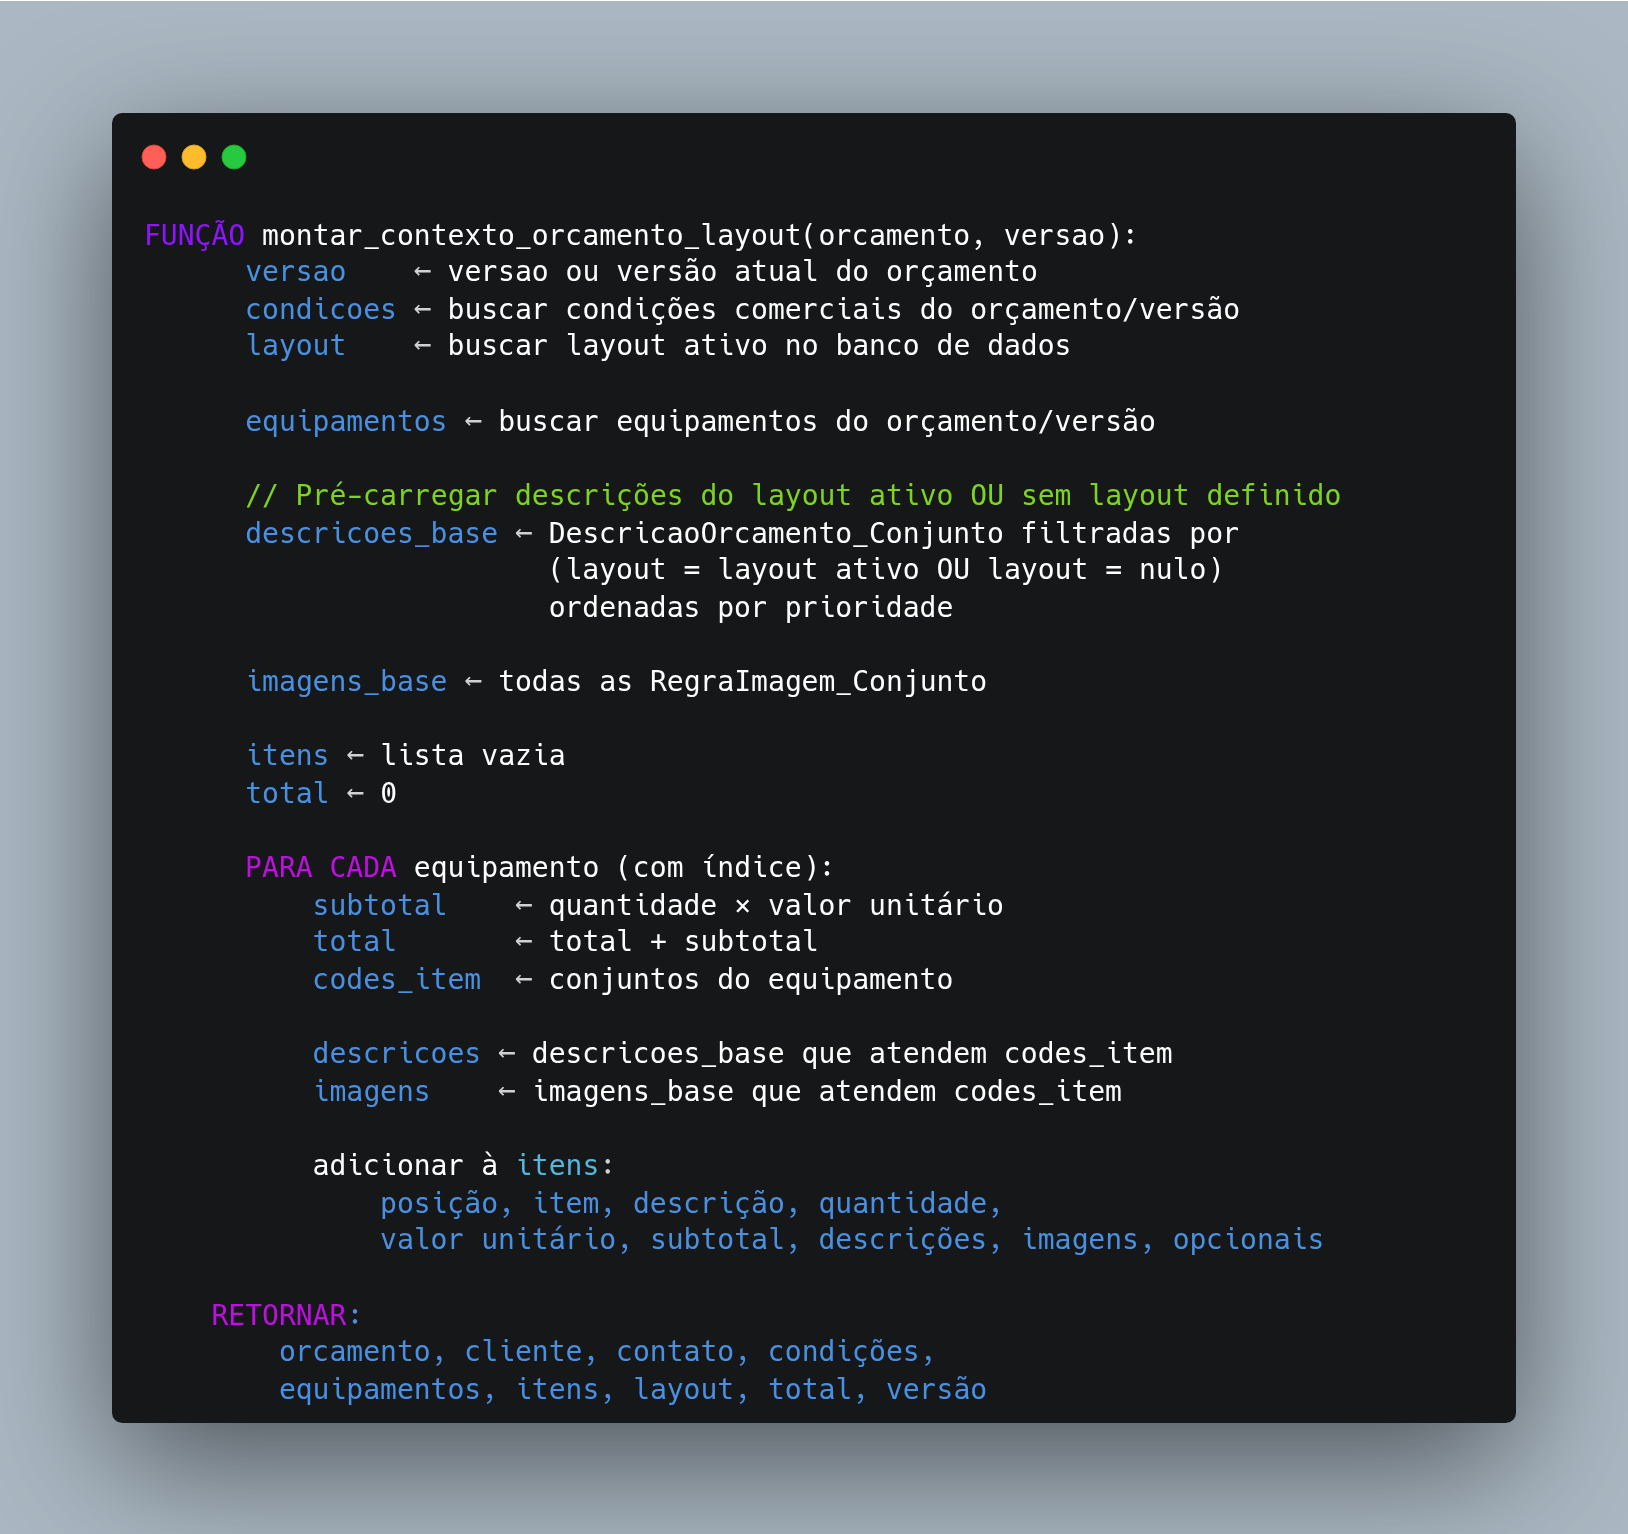
\includegraphics[width=0.90\textwidth]{figuras/05-desenvolvimento/Pseudo Código/funçãomontarcontexto.png}
    \legend{Fonte: Própria do autor (2026), elaborado com Carbon (carbon.now.sh).}
\end{figure}

\subsubsection{Função orcamento\_layout\_pdf\_view}

A função \texttt{orcamento\_layout\_pdf\_view} é a \textit{view} principal, responsável por
orquestrar todo o pipeline de geração. Recebe a requisição HTTP, o identificador do orçamento e
a versão, e executa a seguinte sequência: localiza o orçamento no banco de dados; resolve o layout
ativo e o diretório de trabalho do template; monta o contexto de dados; renderiza o template
\texttt{main.tex} com as variáveis substituídas; salva o arquivo \texttt{.tex} renderizado em disco;
aciona o compilador LuaLaTeX via \texttt{latexmk}; e retorna o PDF gerado como resposta HTTP.
Cada etapa possui tratamento de erro individual: ausência de layout ativo, arquivo ZIP não
encontrado, template ausente ou falha na compilação resultam em resposta 404 com registro do
erro no terminal. A \autoref{fig:funcao-view} apresenta o pseudocódigo da função.

\begin{figure}[htb]
    \caption{\label{fig:funcao-view}Estrutura e lógica da função \texttt{orcamento\_layout\_pdf\_view}}
    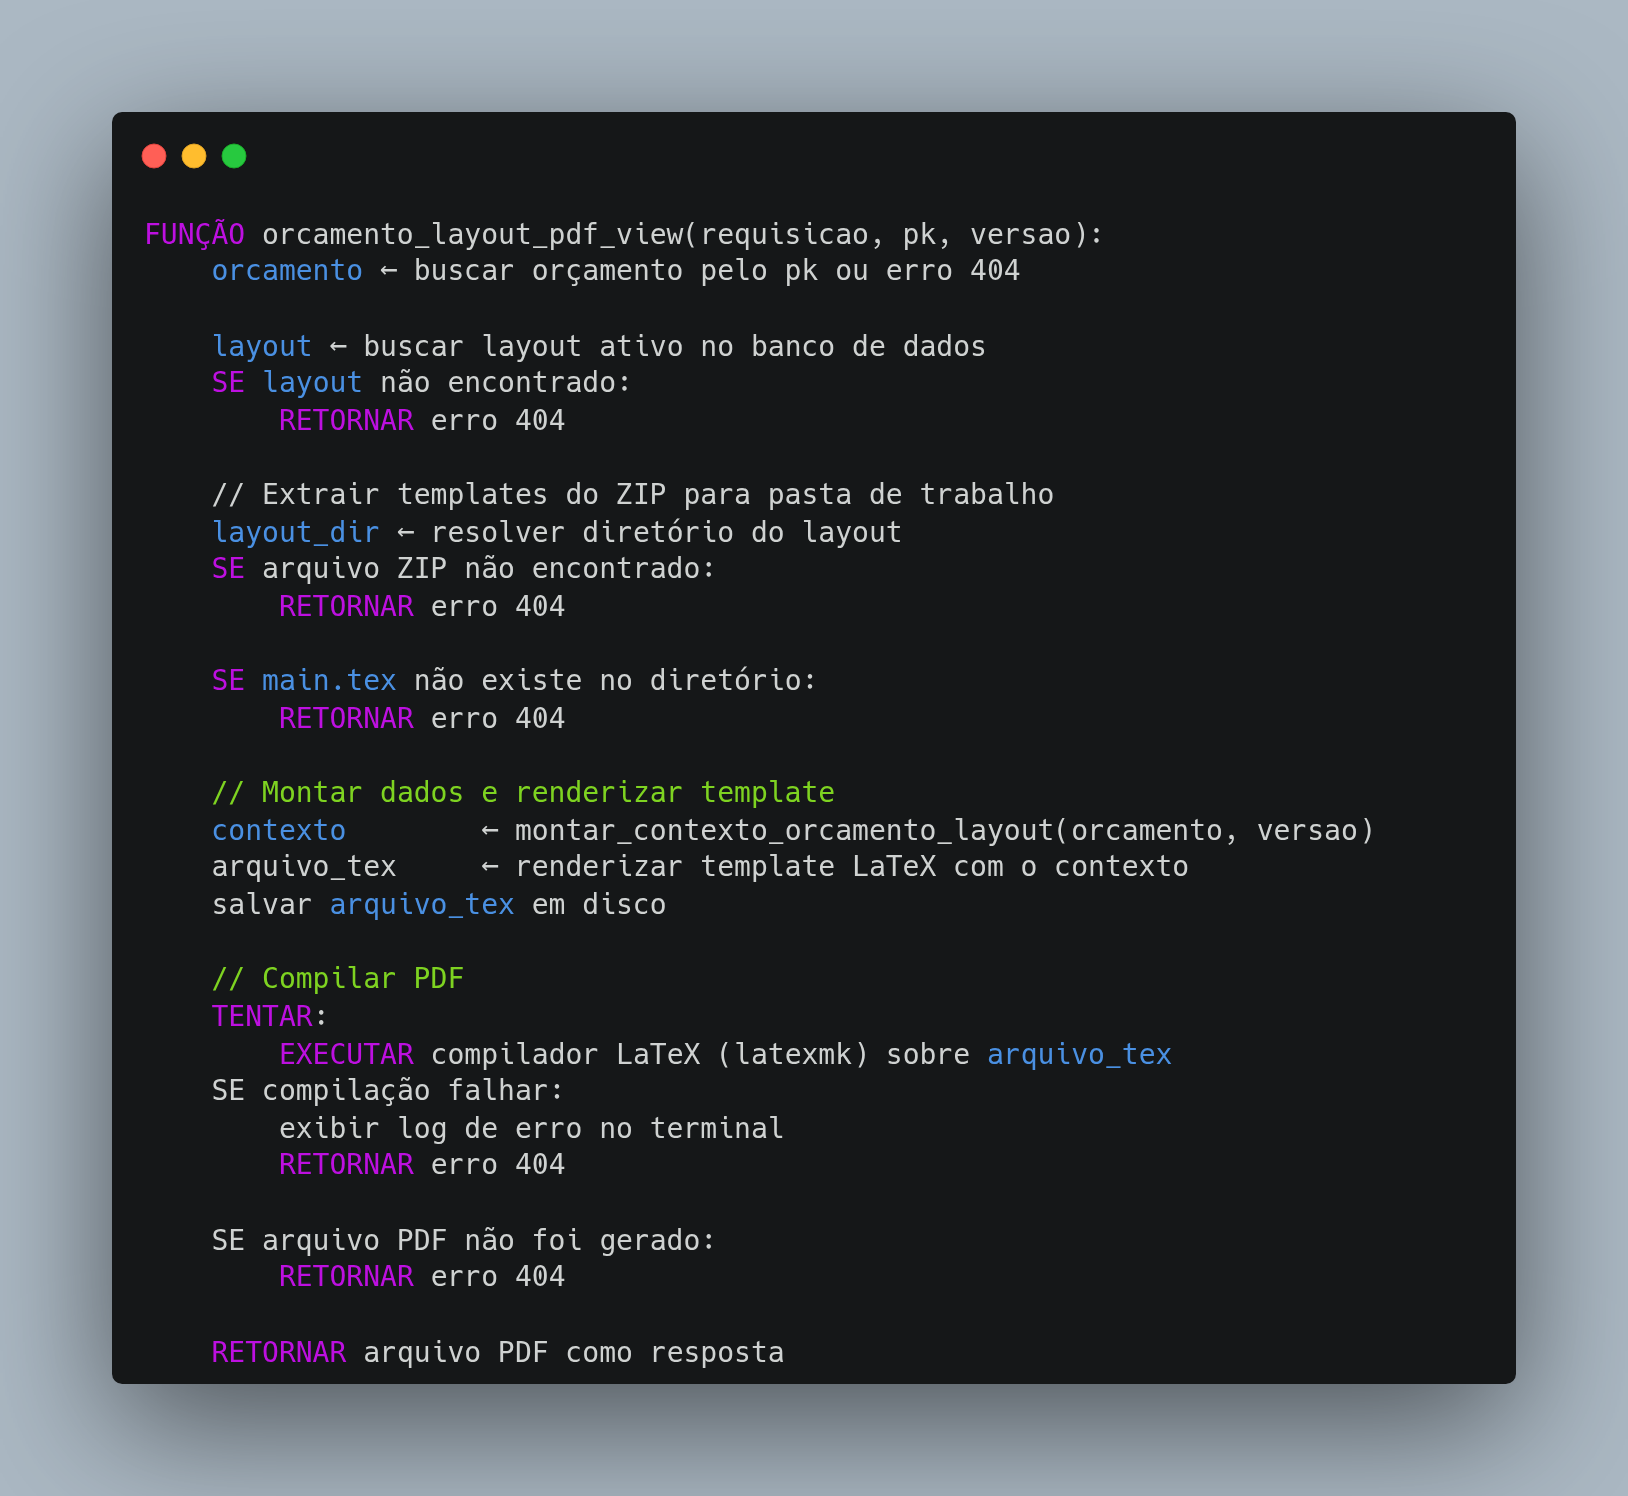
\includegraphics[width=0.90\textwidth]{figuras/05-desenvolvimento/Pseudo Código/FunçãoOrcamento_layout_pdf_view.png}
    \legend{Fonte: Própria do autor (2026), elaborado com Carbon (carbon.now.sh).}
\end{figure}

\subsection{Integração com o Django Admin}

O modelo \texttt{LayoutOrcamento} foi registrado no painel administrativo do Django, permitindo que
gestores realizem o upload de novos templates (\texttt{.zip}) e ativem um layout diretamente pela
interface web, sem qualquer interação com o código-fonte. Ao marcar o campo \texttt{is\_active}
como verdadeiro em um registro, o método \texttt{save()} sobrescrito desativa automaticamente
todos os demais layouts antes de salvar, garantindo a consistência do estado ativo único.

%-------------------------------------------------
\section{Resultados e Discussões}
%-------------------------------------------------
\label{sec:resultados}

Ao final do período de estágio, o pipeline de geração de orçamentos com o novo layout estava funcional
em ambiente de desenvolvimento: o template LaTeX era renderizado corretamente pelo sistema de templates
do Django e compilado com sucesso pelo \texttt{latexmk}, produzindo o PDF com o layout definido pela
empresa de design. A injeção das variáveis de contexto, dados do cliente, itens, descrições técnicas
e condições comerciais, estava em fase de validação final antes da integração ao ambiente de produção.

O Quadro~\ref{qdr:comparativo} apresenta uma comparação entre o sistema legado (PyLaTeX) e a nova
arquitetura implementada.

\begin{quadro}[htb]
    \caption{\label{qdr:comparativo}Comparativo entre o sistema legado e o sistema desenvolvido}
    \begin{tabular}{|p{4.5cm}|p{4.5cm}|p{4.5cm}|}
        \hline
        \textbf{Aspecto} & \textbf{Sistema Legado (PyLaTeX)} & \textbf{Novo Sistema (Django + \LaTeX)} \\
        \hline
        Alteração de layout & Requer modificação de código Python & Realizada via painel administrativo \\
        \hline
        Suporte a múltiplos layouts & Não & Sim, com ativação dinâmica \\
        \hline
        Descrições técnicas por conjunto & Não estruturado & Gerenciadas via modelo dedicado \\
        \hline
        Qualidade tipográfica & Limitada pela abstração da biblioteca PyLaTeX & Total controle via \LaTeX{} nativo \\
        \hline
        Separação de responsabilidades & Baixa (layout no código) & Alta (layout no template) \\
        \hline
    \end{tabular}
    \legend{Fonte: Própria do autor (2026).}
\end{quadro}

A decisão arquitetural de resolver o layout em tempo de geração --- em vez de persistir a referência
no modelo \texttt{Orcamento} --- mostrou-se adequada: manteve o modelo de negócio limpo e permitiu
que a troca de layout afete todas as gerações futuras sem exigir alterações em registros históricos.
A principal ressalva é que orçamentos gerados em momentos diferentes poderão ter layouts distintos,
o que é aceitável no contexto operacional da empresa e pode ser tratado futuramente com o
armazenamento do PDF gerado associado ao registro do orçamento.

O tratamento do conflito de delimitadores entre Django e \LaTeX{}, validado pela referência ao padrão
já utilizado no módulo de inspeção (\texttt{viewsinspecao.py}), demonstrou que a solução é extensível
a qualquer template \LaTeX{} processado pelo sistema, consolidando um padrão técnico reaproveitável
por toda a aplicação.
% ==============================================================================
% CAPÍTULO 6 - CONSIDERAÇÕES FINAIS
% ==============================================================================

\chapter{Considerações Finais}
\label{cap:consideracoes}

O estágio realizado na BIOTECNO Indústria e Comércio Ltda. teve como objetivo central o desenvolvimento
de um módulo de geração automatizada de propostas técnicas e comerciais em PDF, com suporte a layouts
intercambiáveis gerenciáveis pelo painel administrativo do Django. O objetivo foi alcançado: ao término
do período, o sistema estava implementado e funcional em ambiente de desenvolvimento, com pipeline de
geração completo da resolução do layout ativo à entrega do PDF compilado pelo LuaLaTeX, pronto
para ser integrado ao ambiente de produção na próxima atualização da aplicação.

%-------------------------------------------------
\section{Conclusões}
%-------------------------------------------------
\label{sec:conclusoes}

A experiência de estágio proporcionou uma imersão em decisões técnicas que raramente se apresentam com
a mesma complexidade e consequência no ambiente acadêmico. A necessidade de integrar dois sistemas com
gramáticas conflitantes, o motor de templates do Django e a sintaxe do LaTeX, exigiu compreensão
profunda de como cada camada funciona internamente, indo além do uso superficial das ferramentas. Da
mesma forma, a decisão de não acoplar o layout ao modelo \texttt{Orcamento} foi fruto de uma análise
de \textit{trade-offs} reais: entre consistência histórica e flexibilidade operacional, optou-se pela
flexibilidade — decisão validada pelo contexto de negócio da empresa.

Do ponto de vista técnico, o estágio consolidou conhecimentos em Django ORM, modelagem relacional,
geração de documentos com LaTeX e integração de processos externos via \texttt{subprocess}, conteúdos
abordados no curso de Ciência da Computação e que, no contexto prático, revelaram nuances e
interdependências não evidentes na teoria. A leitura e compreensão de um sistema de software já em
produção, com múltiplos módulos, convenções próprias e histórico de decisões acumulado, foi por si só
um aprendizado valioso para a formação profissional.

Do ponto de vista comportamental, a dinâmica de trabalho com ciclos curtos de revisão junto ao
supervisor reforçou a importância da comunicação técnica clara e da validação incremental de decisões
de arquitetura. Erros foram identificados e corrigidos precocemente, evitando retrabalho de maior
escala.

Um aspecto relevante que o estágio evidenciou, e que raramente é abordado no ambiente acadêmico,
é a prática de substituição progressiva de código legado por soluções mais modernas e padronizadas.
A migração do módulo de orçamentos do PyLaTeX para a arquitetura de templates Django não foi motivada
por uma falha crítica do sistema anterior, mas pela necessidade de padronização interna e pela
oportunidade de tornar o sistema mais sustentável a longo prazo. Identificar esse tipo de demanda,
propor uma solução arquitetural coerente e executá-la sem quebrar o que já funcionava é uma habilidade
que a formação acadêmica prepara teoricamente, mas que só se desenvolve plenamente na prática.

Por fim, o fato de já atuar na empresa de forma remunerada antes do início do estágio
curricular teve impacto direto na produtividade e na qualidade das entregas. O conhecimento prévio
do sistema Bioweb, das convenções de código adotadas pela equipe e da estrutura do projeto eliminou
a curva de ambientação inicial, permitindo que o desenvolvimento começasse com foco imediato no
problema técnico. Essa familiaridade também facilitou a leitura de módulos existentes como referência, como o uso do \texttt{viewsinspecao.py} para resolver o conflito de delimitadores Django e
\LaTeX{}, acelerando decisões que, em outro contexto, exigiriam investigação mais prolongada.

%-------------------------------------------------
\section{Trabalhos Futuros}
%-------------------------------------------------
\label{sec:trabalhos-futuros}

A continuidade natural do trabalho desenvolvido aponta para os seguintes encaminhamentos:

\begin{itemize}
    \item \textbf{Publicação em produção}: integrar o novo sistema de geração ao ambiente de produção
    da aplicação, substituindo definitivamente a função legada baseada em PyLaTeX, após validação
    completa das variáveis de contexto com dados reais;
    \item \textbf{Múltiplos layouts por tipo de venda}: ampliar o modelo \texttt{LayoutOrcamento} para
    suportar diferentes layouts por categoria de venda (direta, licitação, revenda), permitindo que a
    seleção do template seja automatizada com base nos atributos do orçamento;
    \item \textbf{Interface de pré-visualização}: desenvolver uma funcionalidade de pré-visualização
    do PDF no painel administrativo antes da ativação de um novo layout, reduzindo o risco de
    publicação de templates com erros de formatação.
\end{itemize}

% ==========================================================================
% ELEMENTOS PÓS-TEXTUAIS
% ==========================================================================
\postextual

% --- Referências bibliográficas ---
\bibliography{referencias}

% --- Apêndices ---
%\begin{apendicesenv}
    % %Imprime uma página indicando o início dos apêndices
    % \partapendices

%    \input{apendices/apendice-a}
%\end{apendicesenv}

% --- Anexos ---
\begin{anexosenv}
    % %Imprime uma página indicando o início dos anexos
     \partanexos
    % ==============================================================================
% ANEXO A - Template de Proposta Comercial
% ==============================================================================

\chapter{Template de Proposta Comercial}
\label{anx:anexo-a}

A seguir, apresenta-se o template de proposta técnica e comercial gerado pelo sistema desenvolvido
durante o estágio, com o layout produzido pela empresa de design e codificado em \LaTeX{} pelo autor.

\includepdf[pages=-]{anexos/orcamento.pdf}
\end{anexosenv}

% --- Índice remissivo (opcional) ---
% \phantompart
% \printindex

\end{document}